% =============================================================================
% Appendix: Supplementary Material
% =============================================================================
% SPDX-FileCopyrightText: 2026 Frank Langbein <frank@langbein.org>
% SPDX-License-Identifier: LPPL-1.3c
%
% Appendices hold supporting material (detailed tables, derivations, survey text,
% user-study materials) so the main narrative stays focused. Complete source
% code is usually submitted separately, not in the report. Use \chapter and
% \section as in main chapters. Replace with your own supplementary material.
% =============================================================================

This appendix contains the supporting material that would interrupt the flow of the main chapters: the \gls{csplib} parser regular expression with worked examples, the derivation of the Big-M constants used in the linearised degree constraints of Section~\ref{subsec:degree-constraints}, and the full per-class output of the candidate generator.

\section[CSPLib Prolog parser]{\gls{csplib} Prolog parser}\label{app:parser}

The parser used in Section~\ref{subsec:data-structures-parsing} consumes the standard \gls{csplib} Prolog format published with Problem 014. Each instance is a single \verb|problem(...)| term with five comma-separated fields: an instance identifier, a fleet specification, a row tally vector, a column tally vector, and a list of hints with one-indexed coordinates.

A representative instance from \verb|data/csplib.pl|:
\begin{verbatim}
    problem(113,
        [4:1,3:2,2:3,1:4],
        [2,4,3,3,2,4,1,1,0,0],
        [0,5,0,2,2,3,1,3,2,2],
        [c@[7,10],w@[1,6]]).
\end{verbatim}

The five fields are extracted by a single compiled regular expression. Whitespace is tolerated around all commas, brackets, and parentheses; the inner lists may be empty (in which case the puzzle has no hints):
\begin{verbatim}
    pattern = re.compile(
        r'problem\s*\(\s*(\d+)\s*,'      # instance id
        r'\s*\[(.*?)\]\s*,'              # fleet
        r'\s*\[(.*?)\]\s*,'              # row tallies
        r'\s*\[(.*?)\]\s*,'              # column tallies
        r'\s*\[(.*?)\]\s*\)\.',          # hints
        re.DOTALL
    )
\end{verbatim}

Hints are then extracted from the fifth capture group with a secondary regular expression \verb|([wcmlrtb])@\[\s*(\d+)\s*,\s*(\d+)\s*\]|. \gls{csplib} uses one-indexed coordinates throughout, which the parser converts to zero-indexed coordinates before constructing the \verb|BattleshipPuzzle| object.

\section{Big-M Derivation for the Linearised Degree Constraints}\label{app:bigm}

The Big-M constants $M = 4$ for the submarine bound, $M = 3$ for the end-piece upper bound, $M = 1$ for the end-piece lower bound, and $M = 2$ for the middle-piece bounds in Section~\ref{subsec:degree-constraints} are not arbitrary. Each is the smallest value that fully deactivates the corresponding constraint when its indicator is zero, given the bound $0 \leq \eta_{i,j} \leq 4$.

\textbf{Submarine Bound:}
The constraint $\eta_{i,j} \leq M (1 - v_{i,j}^c)$ must be a no-op when $v_{i,j}^c = 0$, i.e. it must be implied by $\eta_{i,j} \leq |\mathcal{N}(i, j)| \leq 4$ alone. The smallest $M$ satisfying $M \geq \max \eta_{i,j} = 4$ is therefore $M = 4$.

\textbf{End-piece Upper Bound:}
The constraint $\eta_{i,j} \leq 1 + M(1 - e_{i,j})$ must be a no-op when $e_{i,j} = 0$. This requires $1 + M \geq 4$, giving $M \geq 3$, so the smallest valid value is $M = 3$.

\textbf{End-piece Lower Bound:}
The constraint $\eta_{i,j} \geq 1 - M(1 - e_{i,j})$ must be a no-op when $e_{i,j} = 0$. This requires $1 - M \leq 0$, giving $M \geq 1$, so the smallest valid value is $M = 1$.

\textbf{Middle-piece bounds.}
For both the upper bound $\eta_{i,j} \leq 2 + M(1 - v_{i,j}^m)$ and the lower bound $\eta_{i,j} \geq 2 - M(1 - v_{i,j}^m)$ to be no-ops when $v_{i,j}^m = 0$, we require $2 + M \geq 4$ and $2 - M \leq 0$, both giving $M \geq 2$. The smallest valid value is therefore $M = 2$ on both sides.

Choosing the smallest valid $M$ matters: a tighter Big-M produces a tighter linear-programming relaxation, which strengthens the bounds Gurobi computes at the root node and reduces the cuts it has to add downstream.

\section{Candidate Generator Output for the Standard Fleet}\label{app:candidate-counts}

The Ship Model's pre-processing routine of Section~\ref{subsec:pre-proc-and-candidate-gen} enumerates every geometrically valid ship placement on an $N \times N$ grid for each fleet class $L \in F$. For the standard \gls{csplib} fleet $F = \{4{:}1, 3{:}2, 2{:}3, 1{:}4\}$ the per-class counts on a $10 \times 10$ grid are:

\begin{table}[h]
  \centering
  \begin{tabular}{lccc}
    \toprule
    Length $L$ & Horizontal placements & Vertical placements & Total \\
    \midrule
    4 & 70 & 70  & 140 \\
    3 & 80 & 80  & 160 \\
    2 & 90 & 90  & 180 \\
    1 (submarines) & 100 & --- & 100 \\
    \midrule
    \multicolumn{3}{r}{Grand total $|\mathcal{C}|$:} & 580 \\
    \bottomrule
  \end{tabular}
  \caption{Per-class candidate counts for the standard \gls{csplib} fleet on a $10 \times 10$ grid. Submarines are recorded only once because their orientation is irrelevant. Total of 580 candidates matches the test assertion in \texttt{src/solver\_utils.py}.}
\end{table}

The generator's growth rate is $\mathcal{O}(N^2 L_{\max})$ across all fleet classes combined. On the $30 \times 30$ scaled fleet this rises to several thousand candidates, which is the primary source of the Ship Model's memory footprint discussed in Section~\ref{subsec:hardware-memory-ceilings}.

\section{Graphical User Interface}\label{app:gui}

The CustomTkinter front-end (Section~\ref{subsec:core-sys-modules}, layer 3) provides two interaction modes via a tab strip: a Batch Evaluation tab for running the full benchmark pipeline against a Prolog dataset file, and a Single Puzzle Solver tab for interactive construction and solving of individual instances. Both tabs share the thread-safe message-passing infrastructure described in Section~\ref{subsec:platform-challenges-thread-safety}.

\begin{figure}[h]
  \centering
  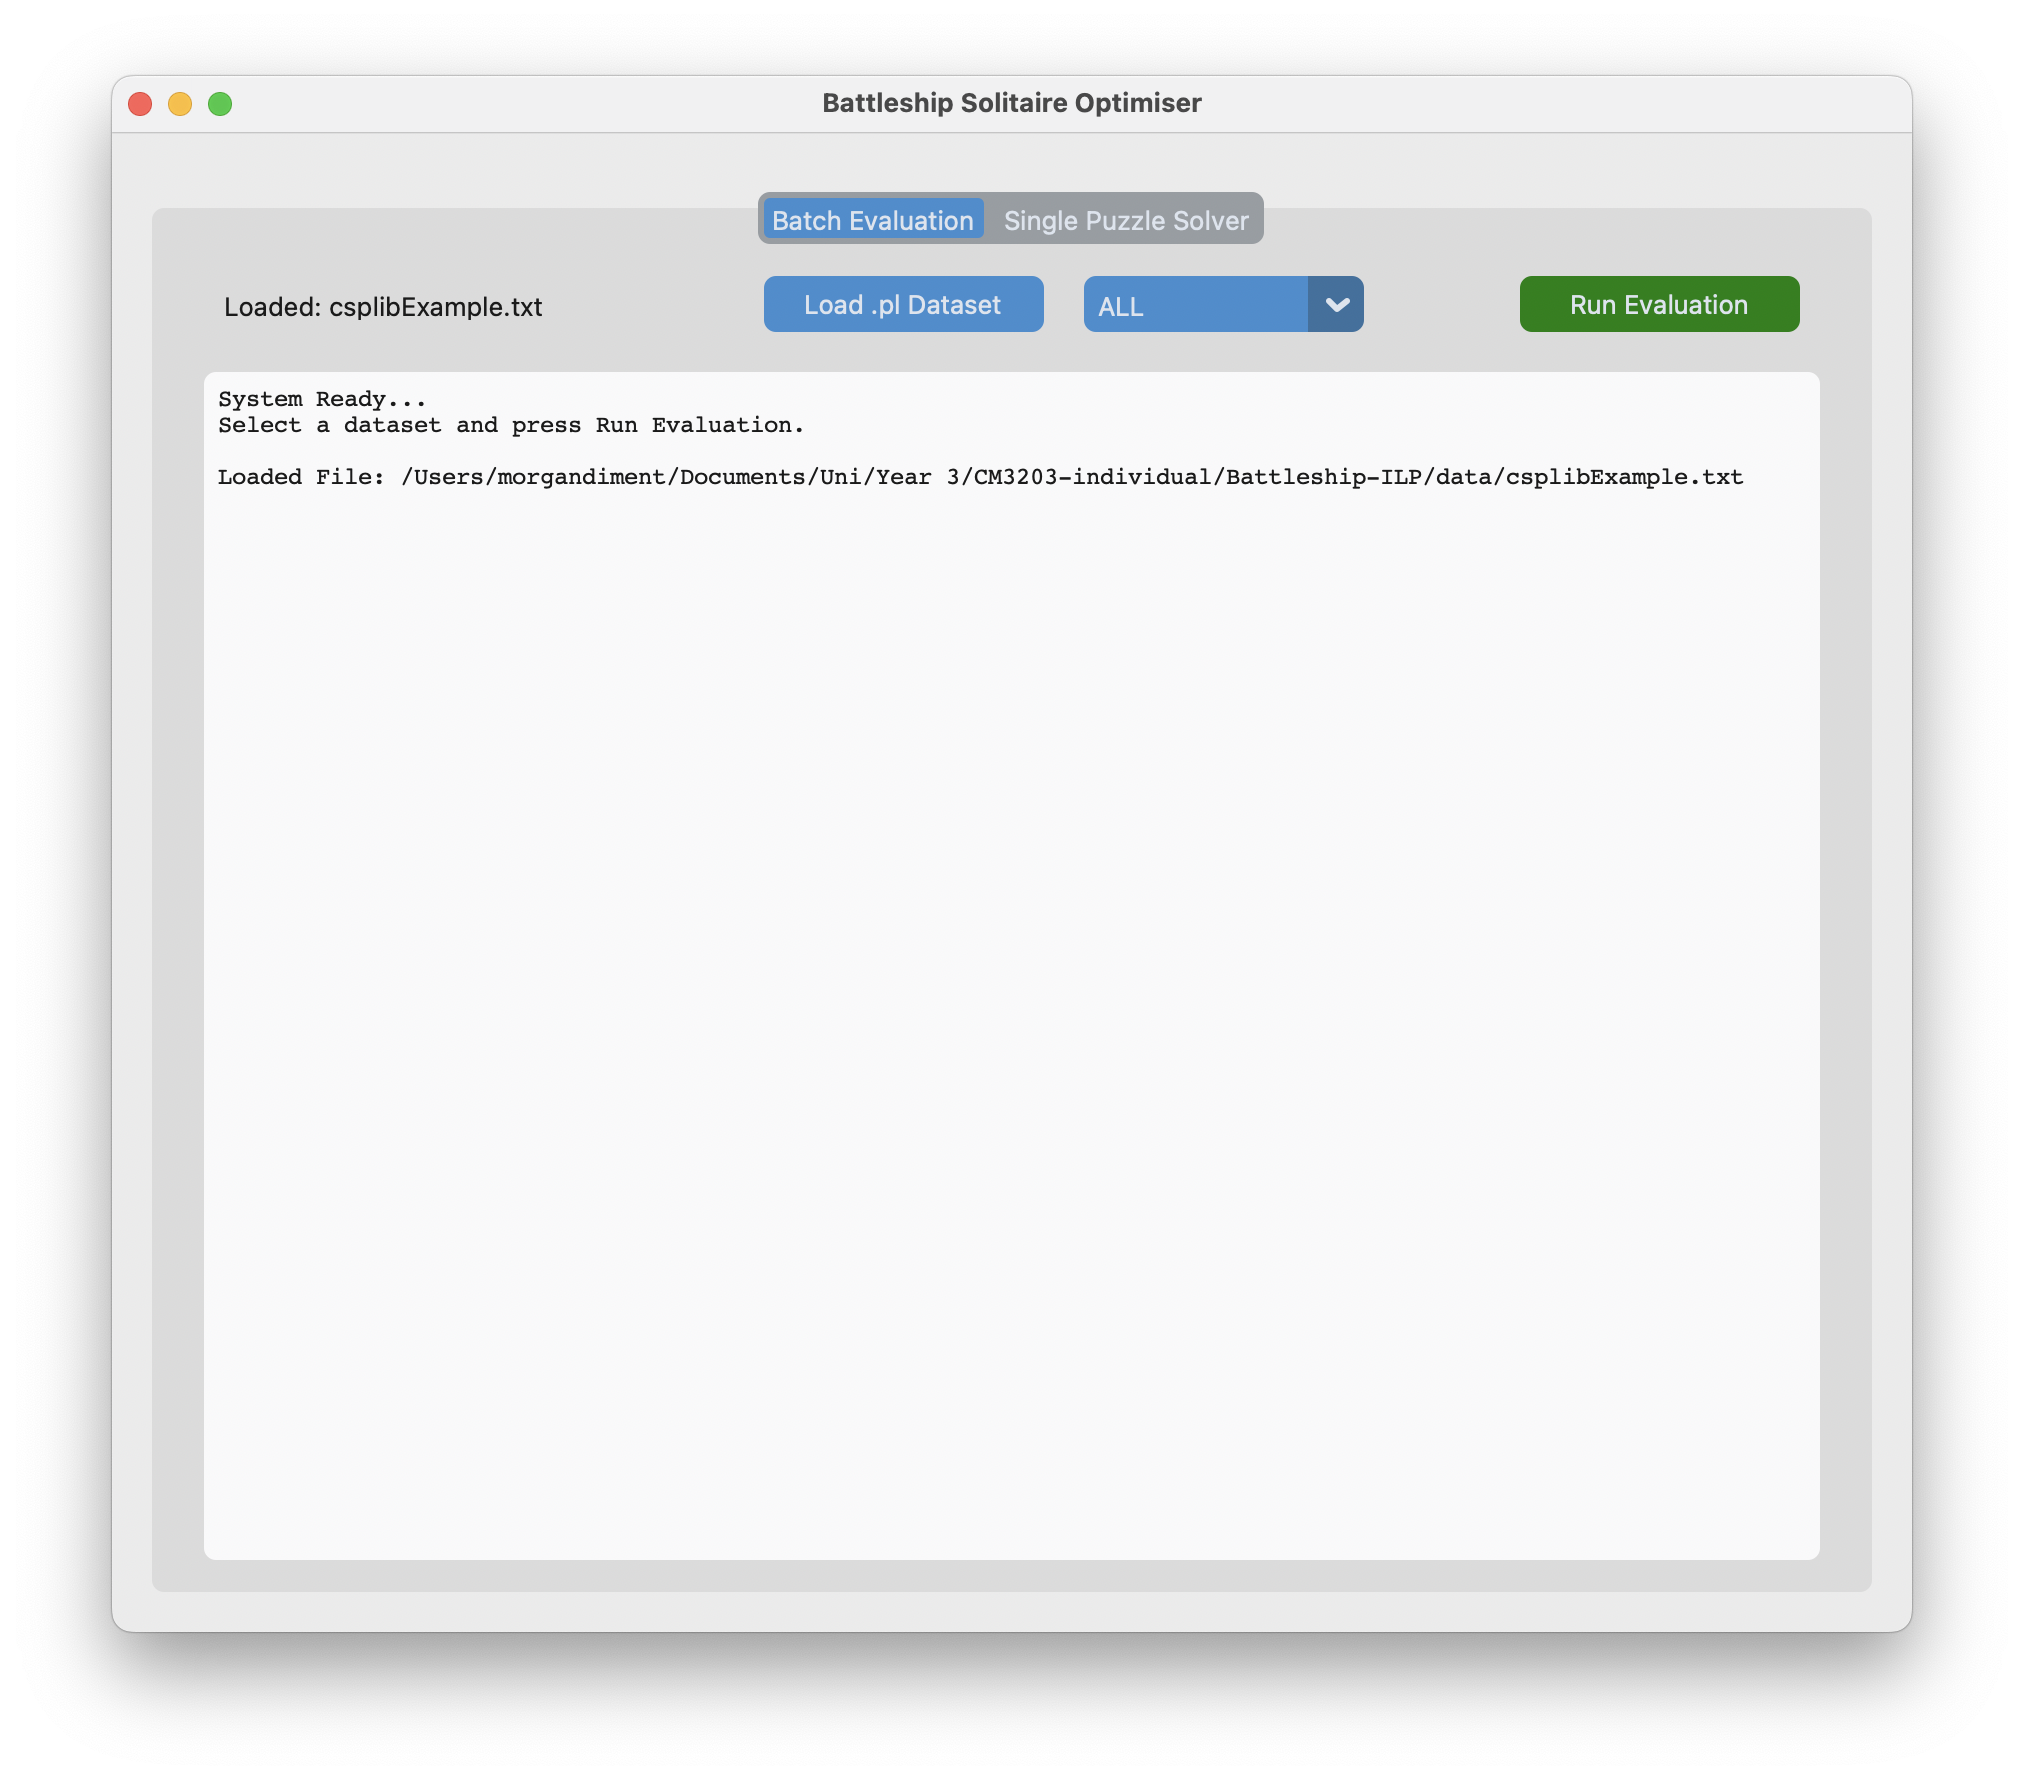
\includegraphics[width=0.95\linewidth]{images/GUI/batch-tab.png}
  \caption{Batch Evaluation tab. The user loads a Prolog dataset file (left), selects which solver(s) to run from the drop-down (centre), and presses ``Run Evaluation''. The console pane streams the per-instance comparison table as the evaluator processes each puzzle, with output marshalled from the background solver thread to the main UI thread through the \texttt{TextboxRedirector} class.}
  \label{fig:gui_batch}
\end{figure}

\begin{figure}[h]
  \centering
  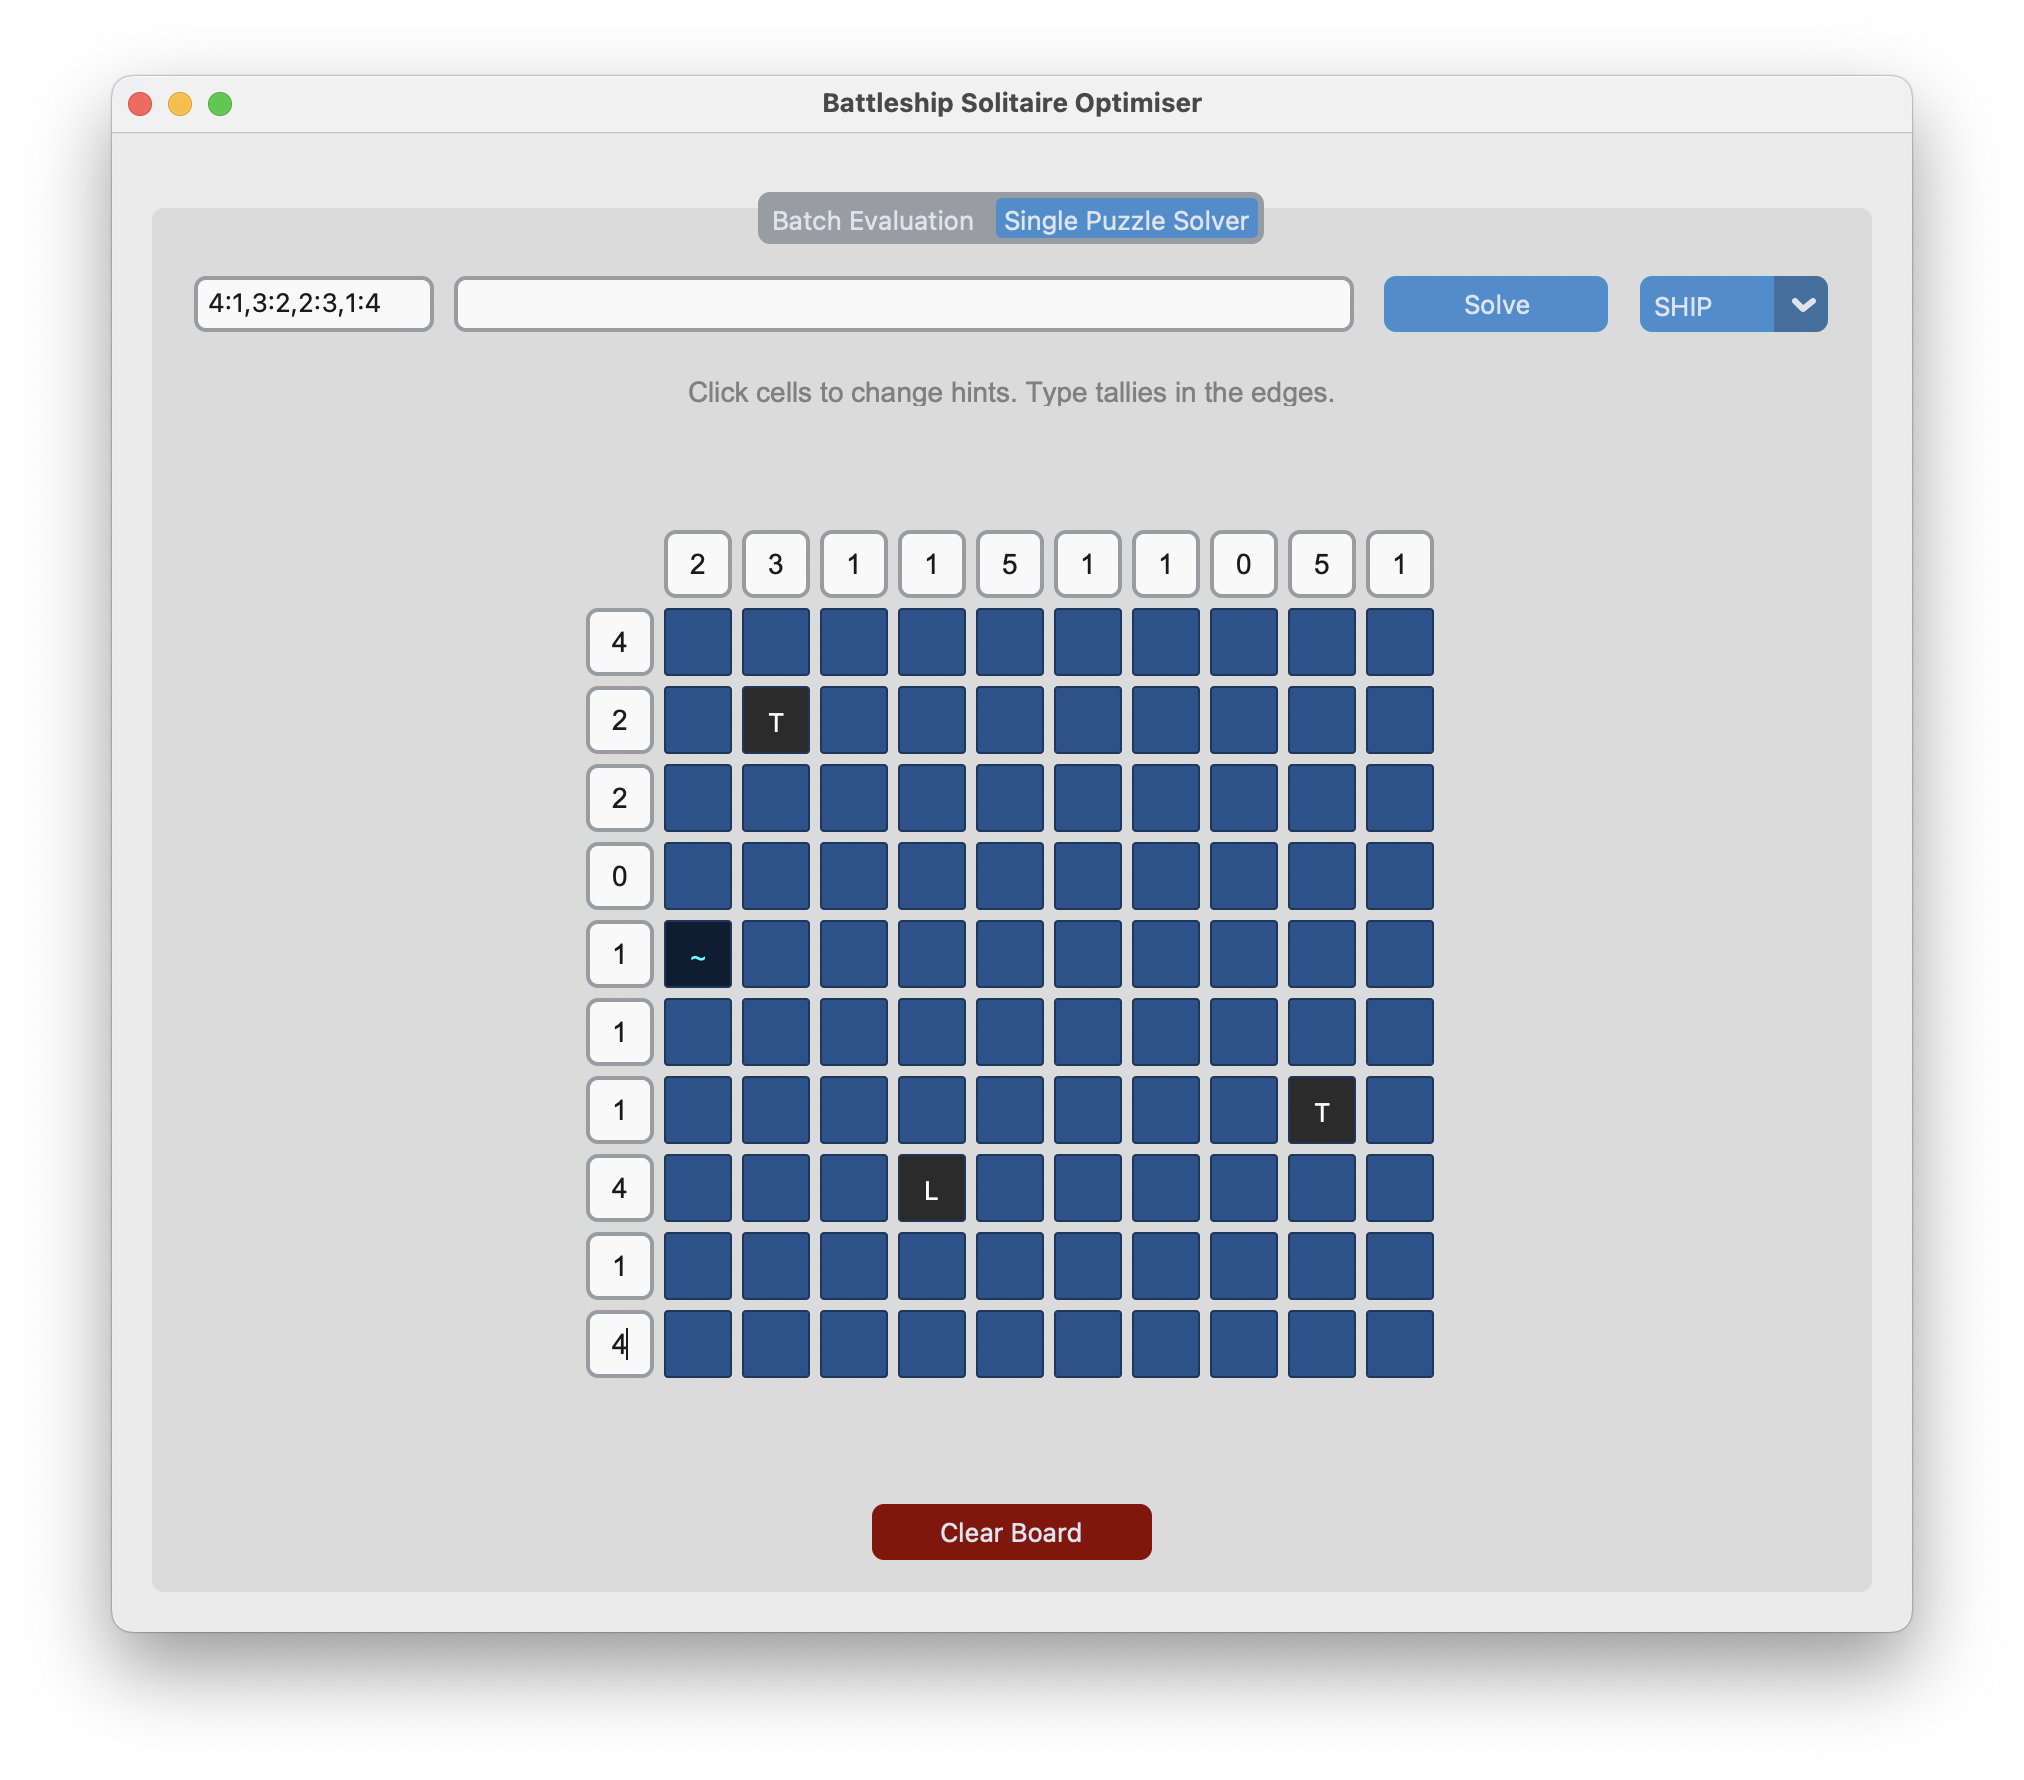
\includegraphics[width=0.95\linewidth]{images/GUI/single-puzzle-unsolved.png}
  \caption{Single Puzzle Solver tab in input mode. The fleet specification, row tallies and column tallies are typed into the bordered input boxes; clicking each grid cell cycles through the seven possible \gls{csplib} states (water, submarine, top, bottom, left, right, middle) for entering hints. The ``Solve'' button dispatches the constructed instance to the chosen solver on a background thread.}
  \label{fig:gui_single_unsolved}
\end{figure}

\begin{figure}[h]
  \centering
  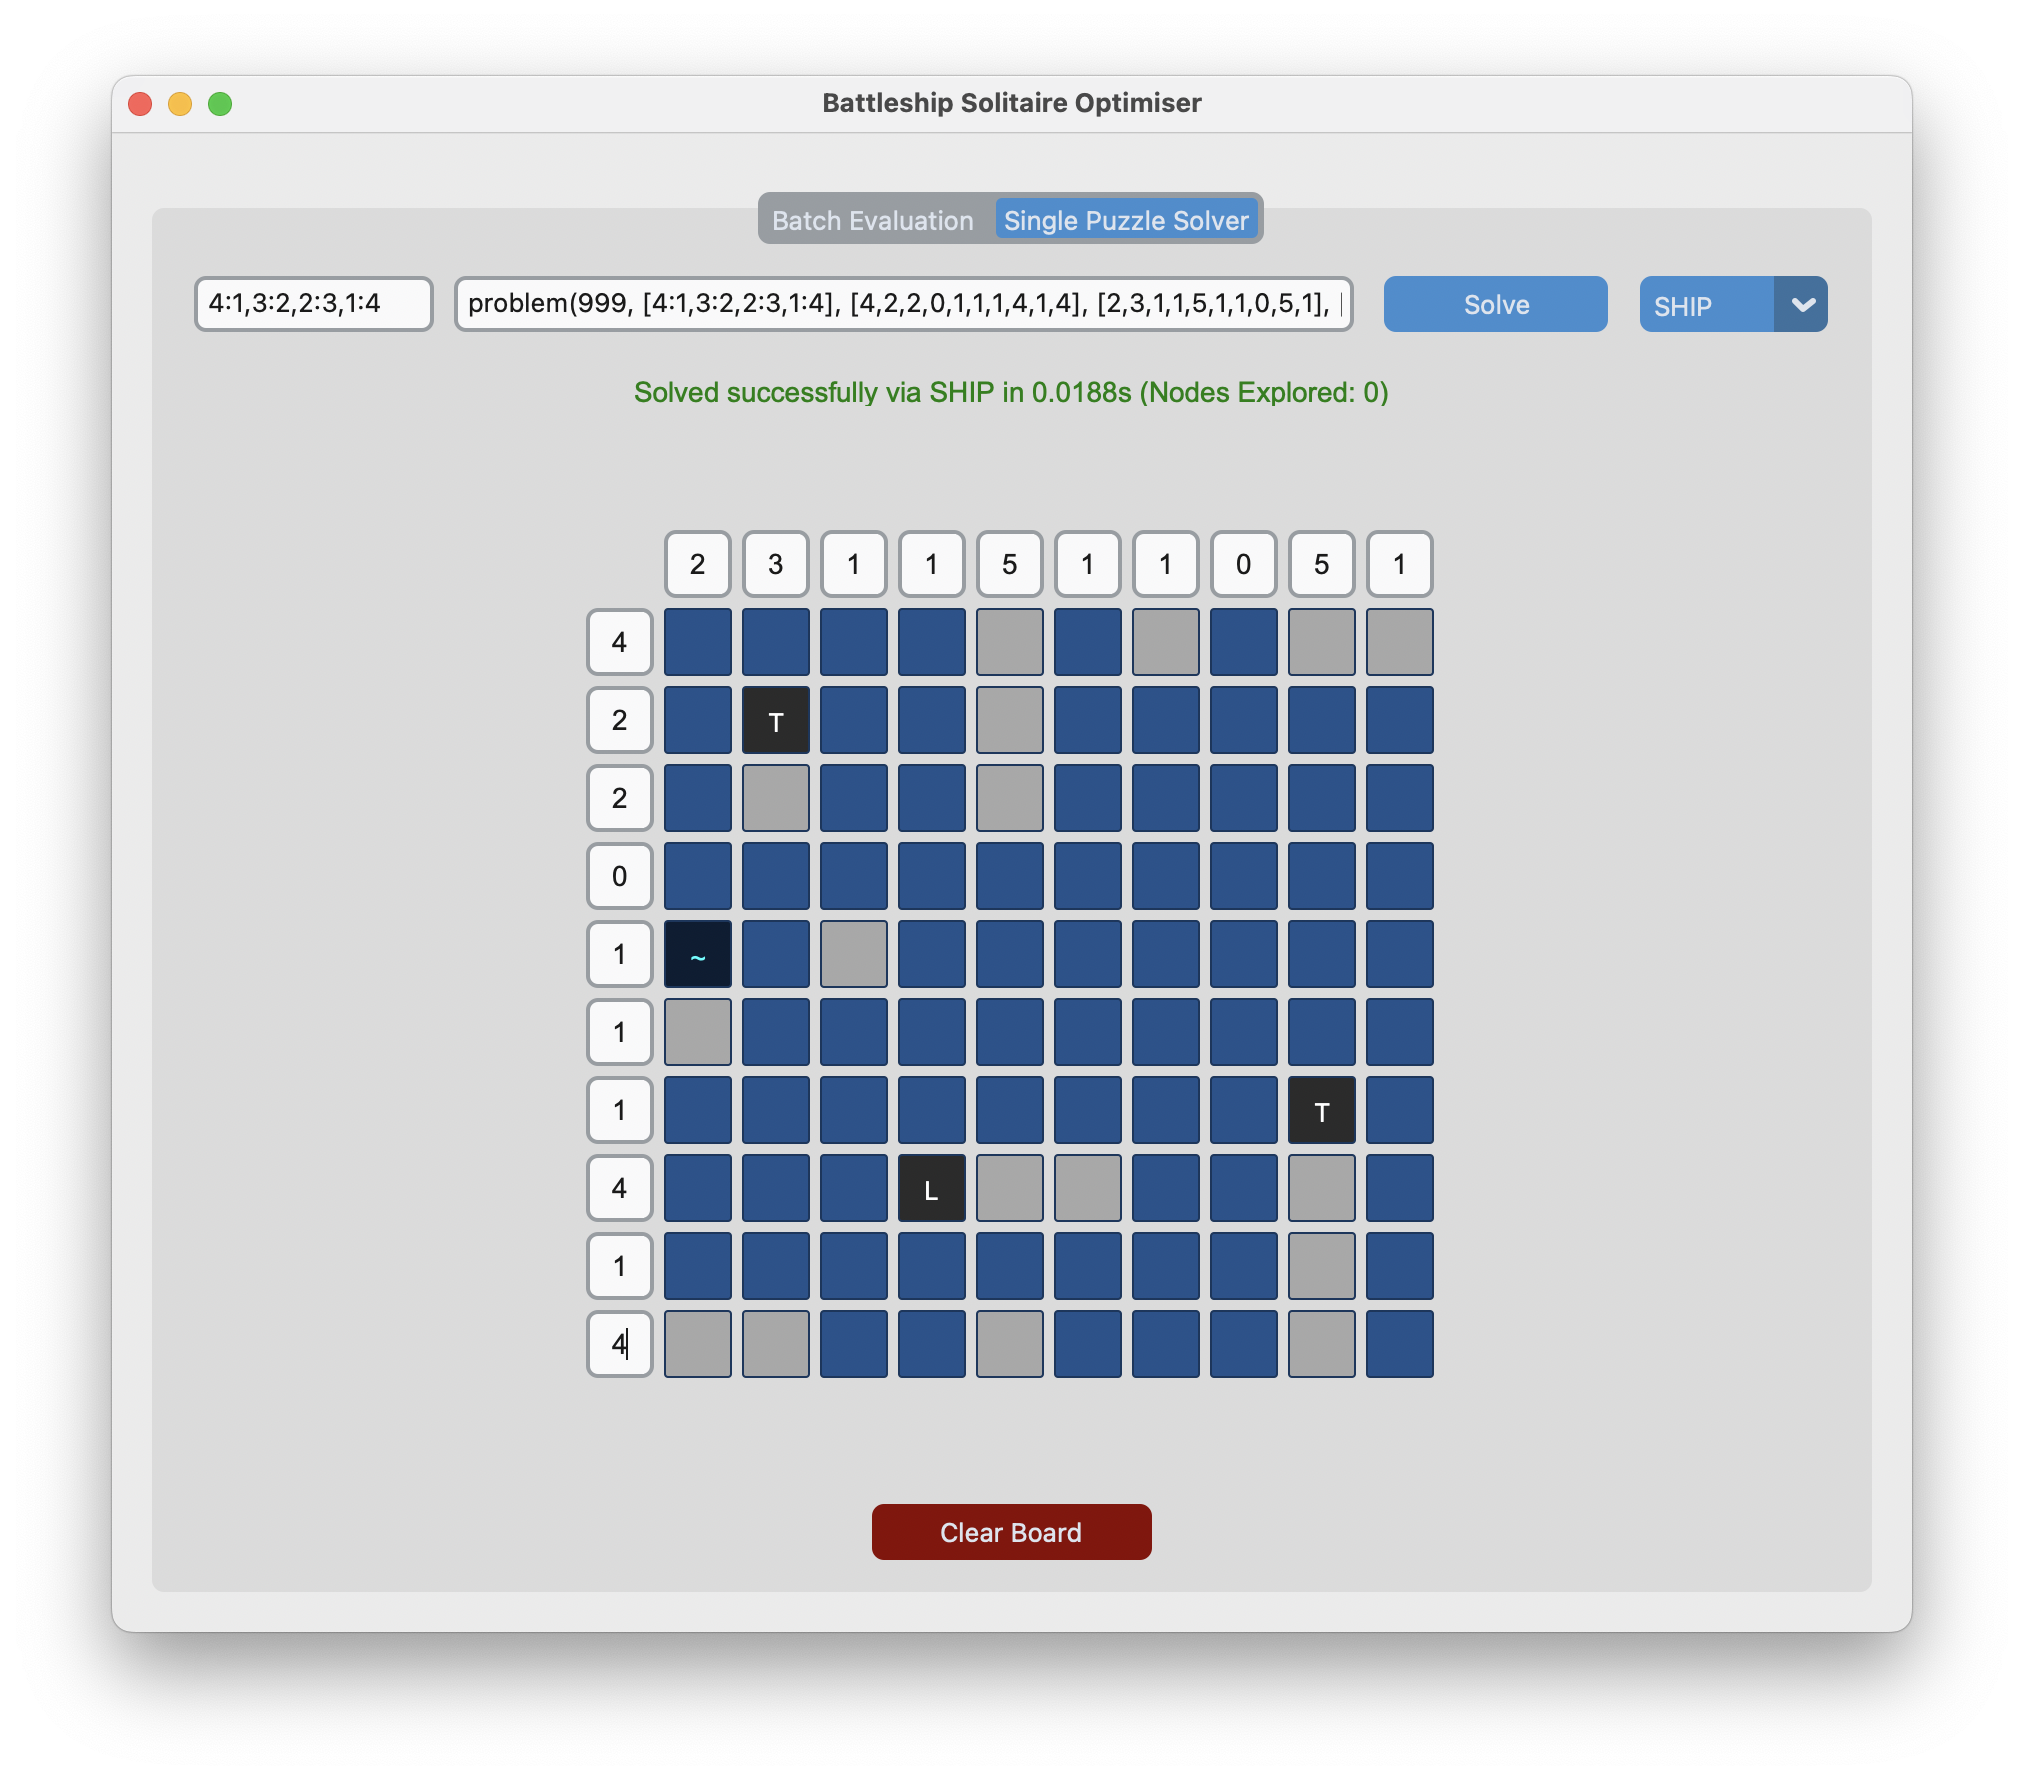
\includegraphics[width=0.95\linewidth]{images/GUI/single-puzzle-solved.png}
  \caption{Single Puzzle Solver tab after solving. The status line reports the wall-clock solve time and the branch-and-bound node count returned by Gurobi. Cells that were not part of the input hint set are repainted in light grey to show the recovered ship placements, and the original hints retain their input colouring.}
  \label{fig:gui_single_solved}
\end{figure}